\documentclass[9.4pt]{beamer}

\usepackage[T3,T1]{fontenc}
\usepackage[utf8]{inputenc}
\usepackage[english]{babel}

\usepackage{algpseudocode}
\usepackage{algorithm}
\usepackage{numapde-manifolds}
\usepackage{xcolor}
\usepackage{comment}
\usepackage{varwidth}

\hypersetup{pdfpagemode=FullScreen}

\usetheme{tuc2019}

\mode<article>{\usepackage{beamerarticletuc2019}}



\DeclareSymbolFont{tipa}{T3}{cmr}{m}{n}
\DeclareMathAccent{\invbreve}{\mathalpha}{tipa}{16}

\newcommand{\StatexIndent}[1][3]{%
  \setlength\@tempdima{\algorithmicindent}%
  \Statex\hskip\dimexpr#1\@tempdima\relax}
\algdef{S}[WHILE]{WhileNoDo}[1]{\algorithmicwhile\ #1}%
\makeatother

\title{The Riemannian BFGS Method and its Implementation in Julia}
\author{Tom-Christian Riemer}
\date{18.12.2020}
\institute[TUC]{TU Chemnitz, Research Seminar Scientific Computing}
\titlegraphic{
\includegraphics[height=0.2\textheight]{tuc2019/logo/tuc_green}}
\tucurl{http://www.tu-chemnitz.de/urz/}



\begin{document}

\tucthreeheadlines
\frame{\titlepage}

\begin{frame}{Contents}
    \tableofcontents
\end{frame}

\section{Introduction}

\begin{frame}{Riemannian Optimization}
    Finding a \textbf{minimum} of a real-valued function $f$ on a Riemannian manifold, i.e.
    \begin{equation*}
        \min f(x), \quad x \in \mathcal{M}.
    \end{equation*}\\[1.\baselineskip]
    \begin{center}
        \textbf{Riemannian manifold} = smooth manifold + Riemannian metric. \\[1.\baselineskip]
    \end{center}
    \begin{equation*}
        \mathbb{S}^{n-1} = \{ x \in \mathbb{R}^n \colon \; \lVert x \rVert_2 = 1 \}.
    \end{equation*}
\end{frame}

\begin{frame}{Optimization Methods}
    \textbf{Line search methods} on Euclidean space
    \begin{equation*}
        x_{k+1} = x_k + \alpha_k d_k,
    \end{equation*}
    where $d_k \in \mathbb{R}^n$ and $\alpha_k > 0$ is a stepsize. \\[1.\baselineskip]

    \textbf{Goal}: Adapt unconstrained Euclidean algorithms to functions on $\mathcal{M}$. \\[1.\baselineskip]

    Cannot apply to problems on Riemannian manifolds directly:
    \begin{itemize}
        \item \textbf{Directions?}
        \item \textbf{Addition?}
    \end{itemize}
\end{frame}

\begin{frame}{Tangent Spaces}
    \vspace{-1\baselineskip}\hfill{\tiny{[Absil, Mahony, Sepulchre, 2008]}}
    \begin{center}
        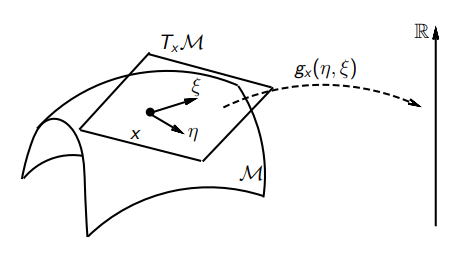
\includegraphics[width=5cm]{img/Riemannian_Metric.png}
    \end{center}
    \textbf{Tangent space} $\tangent{x}$ at $x$, with inner product $g_x(\cdot, \cdot)$. \\[0.2\baselineskip]
    \textbf{Riemannian gradient} $\mathrm{D} \, f(x) [\eta_x] = g_x (\operatorname{grad} f(x), \eta_x), \; \forall \eta_x \in \tangent{x}$. \\[0.2\baselineskip]
    \textbf{Riemannian Hessian} $\operatorname{Hess} f(x) \colon \tangent{x} \to \tangent{x}, \; \eta_x \mapsto \nabla_{\eta_x} \operatorname{grad} f(x)$.
\end{frame}

\begin{frame}{Retractions}
    \vspace{-1\baselineskip}\hfill{\tiny{[Bergmann, 2017]}}
    \begin{center}
        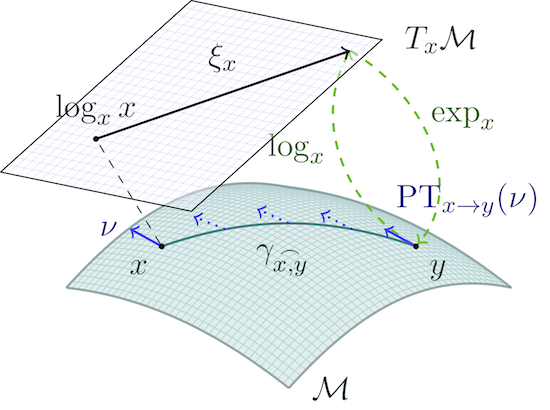
\includegraphics[width=4.5cm]{img/manifold-terms.png}
    \end{center}
    \textbf{Retraction} $R_{x}(\xi_x) \in \mathcal{M}$ with $R_x (0_x) = x$ and $\mathrm{D} \, R_x (0_x)[\xi_x] = \xi_x$.
    \textbf{Geodesic} $\gamma_{\invbreve{x,y}}$ shortest path (on $\mathcal{M}$) between $x$ and $y$. \\[0.2\baselineskip]
    \textbf{Exponential map} $\exponential{x}(\xi_x) = \gamma_{\xi_x}(1)$, where $\gamma_{\xi_x}(0) = x$ and $\dot{\gamma}_{\xi_x}(0) = \xi_x$. \\[0.2\baselineskip]
\end{frame}


\begin{comment}

\begin{frame}{Tangent Space}
    \begin{tabular}{cl}  
        \begin{tabular}{c}
            \parbox{0.6\linewidth}
            {
            \begin{itemize}
                \item Let $\gamma \colon \; I \to \mathcal{M}$ be a curve. A \textbf{tangent vector} $\eta_x$ shows the direction along $\gamma$ at $x$, for which is $\dot{\gamma}(0) = \eta_x$, where $\gamma(0) = x$.
                \item \textbf{Tangent space} at $x$ is the set of all tangent vectors at $x$, denoted by $\tangent{x}$, which is a \textbf{vector space}.
                \item The (disjoint) union of tangent spaces $\tangent{}$ is called \textbf{tangent bundle}.
            \end{itemize}
            }
        \end{tabular}  
        &
        \begin{tabular}{l}
            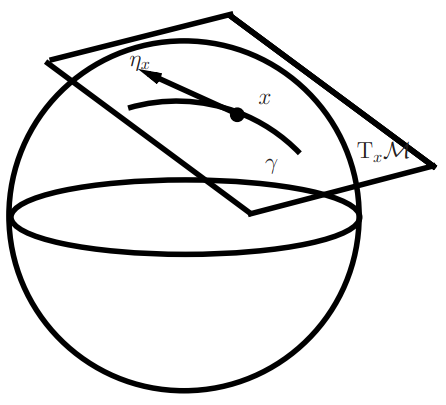
\includegraphics[width=3.5cm]{img/Tangent_Space.png}
        \end{tabular}
    \end{tabular}
\end{frame}

\begin{frame}{Riemannian Metric}
    \begin{center}
        A \textbf{Riemannian metric} $g$ is defined on each $\tangent{x}$ as an inner product $g_x \colon \; \tangent{x} \times \tangent{x} \to \mathbb{R}$. 
    \end{center}
    \begin{tabular}{cl}  
        \begin{tabular}{c}
            \parbox{0.5\linewidth}
            {
            \begin{itemize}
                \item Norms: $\lVert \xi_x \rVert_x = \sqrt{g_x(\xi_x, \xi_x)}$
                \item Orthogonality: $g_x(\xi_x, \eta_x) = 0$
            \end{itemize}
            }
        \end{tabular}  
        &
        \begin{tabular}{l}
            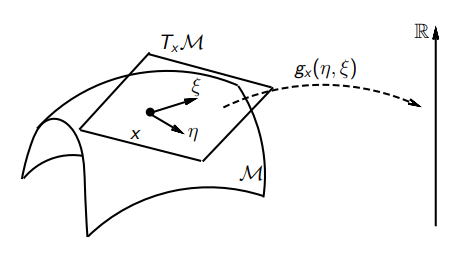
\includegraphics[width=5cm]{img/Riemannian_Metric.png}
        \end{tabular}
    \end{tabular}
    Riemannian distance: $\operatorname{dist}(x,y) = \inf_{\gamma} \bigl\{ \int^{1}_0 \lVert \dot{\gamma}(t) \rVert_{\gamma(t)} \mathrm{d}t \bigr\},$ where $\gamma \colon \; \mathbb{R} \to \mathcal{M}$ is a curve with $\gamma(0) = x$ and $\gamma(1) = y$.
\end{frame}

\begin{frame}{Riemannian Gradient}
    The \textbf{Riemannian gradient} $\operatorname{grad} f$ of $f$ at $x$ is the unique tangent vector such that \begin{equation*} 
        g_x (\operatorname{grad} f(x), \eta_x) = \mathrm{D} \, f(x) [\eta_x], \quad \forall \eta_x \in \tangent{x},
    \end{equation*} 
    where $\mathrm{D} \, f(x) [\eta_x]$ denotes the derivative of $f$ along $\eta_x$. It represents the steepest ascent direction. \\[1.\baselineskip]
    \begin{itemize}
        \item $\eta_{x} \in \tangent{x}$ is a \textbf{descent direction} of $f$ at $x$ if $g_{x} (\operatorname{grad} f(x), \eta_{x}) < 0$.
        \item $x \in \mathcal{M}$ is \textbf{stationary point} of $f$ if $\operatorname{grad}f(x) = 0_x \in \tangent{x}$.
    \end{itemize}
\end{frame}

\begin{frame}{Retractions}
    \begin{tabular}{cl}  
        \begin{tabular}{c}
            \parbox{0.5\linewidth}
            {
                A \textbf{retraction} is a smooth map $R \colon \; \tangent{} \to \mathcal{M}$ with the following properties. Let $R_{x}(\cdot)$ denote the restriction to $\tangent{x}$:
                \begin{itemize}
                    \item $R_x (0_x) = x$,
                    \item and $\mathrm{D} \, R_x (0_x)[\eta_x] = \eta_x$.
                    \item $\gamma(t) = R_{x}(t \; \eta_x) \Rightarrow \dot{\gamma}(0) = \eta_x$.
                    \item $\hat{f}_x (\cdot) = f \circ R_{x}(\cdot) \Rightarrow \operatorname{grad} \hat{f}_x (0_x) = \operatorname{grad} f(x)$.
                \end{itemize}
            }
        \end{tabular}  
        &
        \begin{tabular}{l}
            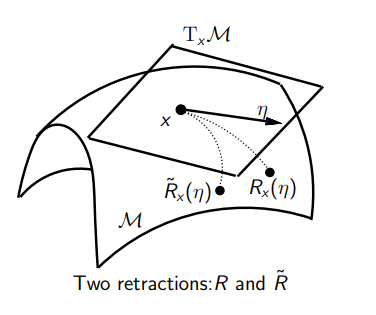
\includegraphics[width=4cm]{img/Retraction.png}
        \end{tabular}
    \end{tabular}
\end{frame}


\begin{frame}{Riemannian Gradient and Riemannian Hessian}
	\begin{itemize}
        \item The \textbf{Riemannian gradient} $\operatorname{grad} f$ of $f$ at $x$ is the unique tangent vector such that \begin{equation*} g_x (\operatorname{grad} f(x), \eta_x) = \mathrm{D} \, f(x) [\eta_x], \quad \forall \eta_x \in \tangent{x}, \end{equation*} where $\mathrm{D} \, f(x) [\eta_x]$ denotes the derivative of $f$ along $\eta_x$. It represents the steepest ascent direction.
        \item The \textbf{Riemannian Hessian} of $f$ at $x$ is a self-adjoint linear operator from $\tangent{x}$ to $\tangent{x}$ defined as \begin{equation*} \operatorname{Hess} f(x) [\eta_x] = \nabla_{\eta_x} \operatorname{grad} f(x), \quad \forall \eta_x \in \tangent{x}, \end{equation*} where $\nabla$ is the Riemannian connection.
    \end{itemize} 
\end{frame}
\end{comment}

\section{Riemannian Quasi-Newton Methods}

\begin{frame}{Riemannian Line Search Methods}
    \begin{equation*}
        x_{k+1} = R_{x_k}(\alpha_k \eta_k)
    \end{equation*}
    where $\eta_k \in \tangent{x_k}$ and $\alpha_k > 0$ is a stepsize. \\[1.\baselineskip]
    \begin{itemize}
        \item Riemannian Newton method: $\eta_k = - {\operatorname{Hess} f(x_k)}^{-1} [\operatorname{grad} f(x_k)]$
        \item \textbf{Riemannian Quasi-Newton methods}: \begin{equation*} \eta_k = - {\mathcal{H}_k}^{-1} [\operatorname{grad} f(x_k)] = - \mathcal{B}_k [\operatorname{grad} f(x_k)] \end{equation*} where $\mathcal{H}_k, \mathcal{B}_k \colon \; \tangent{x_k} \to \tangent{x_k}$ approximates $\operatorname{Hess} f(x_k)$. 
    \end{itemize}
\end{frame}


\begin{frame}{Quasi-Newton Equation}
    Euclidean Case: 
    \begin{equation*}
        H_{k+1} (x_{k+1} - x_k) = \nabla f(x_{k+1}) - \nabla f(x_k)
    \end{equation*} \\[.5\baselineskip]
    Generalization to the Riemannian case: \\[.5\baselineskip]
    \begin{itemize}
        \item $x_{k+1} - x_k$ can be replaced by ${R_{x_k}}^{-1}(x_{k+1})$.
        \item $\operatorname{grad} f(x_k), {R_{x_k}}^{-1}(x_{k+1}) \in \tangent{x_k}$ and $\operatorname{grad} f(x_{k+1}) \in \tangent{x_{k+1}}$ \\ $\Rightarrow$ A method for \textbf{comparing tangent vectors} is required. 
    \end{itemize}
\end{frame}

\begin{frame}{Vector Transports}
    \vspace{-1\baselineskip}\hfill{\tiny{[Bergmann, 2017]}}
    \begin{center}
        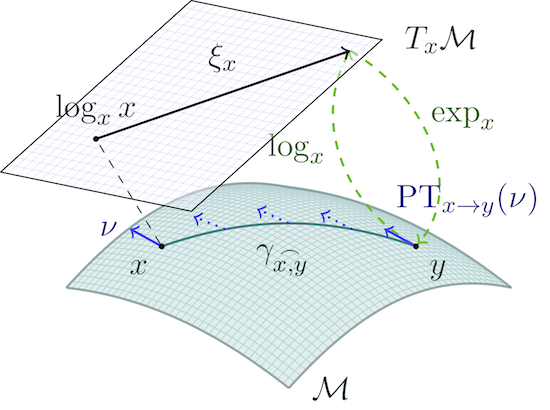
\includegraphics[width=4.5cm]{img/manifold-terms.png}
    \end{center}
    \textbf{Parallel transport} $\mathrm{PT}_{x \rightarrow y} (\nu_x) \in \tangent{y}$ of $\nu_x \in \tangent{x}$ along $\gamma_{\invbreve{x,y}}$. \\[0.15\baselineskip]
    \textbf{VT} $T_{x, \xi_x}(\nu_x) \in \tangent{y}$ with associated retraction $y = R_x(\xi_x)$. \\[0.15\baselineskip]
    \textbf{Isometric VT} satisfies $\lVert \nu_x \rVert_x = \lVert T^{S}_{x, \xi_x}(\nu_x) \rVert_{R_x(\xi_x)}$. \\[0.15\baselineskip]
    \textbf{VT by differentiated retraction} $T^{R}_{x, \xi_x}(\nu_x) = \frac{\mathrm{d}}{\mathrm{d}t} R_{x}(\xi_x + t \; \nu_x) \; \vert_{t=0}$.
\end{frame}


\begin{comment}

\begin{frame}{Vector Transports}
    \begin{tabular}{cl}  
        \begin{tabular}{c}
            \parbox{0.5\linewidth}
            {
                \begin{itemize}
                    \item $T_{x, \eta_x}(\xi_x)$ denotes transport of $\xi_x$ to tangent space of $R_x (\eta_x)$. $R$ is the retraction associated with $T$.
                    \item An isometric vector transport, denoted by $T^S$, additionally satisfies \begin{equation*} g_x (\eta_x, \xi_x) = g_y (T^{S}_{x, \zeta_x}(\eta_x), T^{S}_{x, \zeta_x}(\xi_x))\end{equation*} where $x,y \in \mathcal{M}$, $y = R_x(\zeta_x)$, $\eta_x, \xi_x, \zeta_x \in \tangent{x}$.
                \end{itemize}
            }
        \end{tabular}  
        &
        \begin{tabular}{l}
            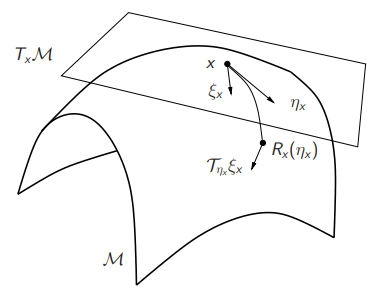
\includegraphics[width=5cm]{img/Vector_Transport.png}
        \end{tabular}
    \end{tabular}
\end{frame}

\begin{frame}{Vector Transport by Differentiated Retraction}
    \begin{tabular}{cl}  
        \begin{tabular}{c}
            \parbox{0.5\linewidth}
            {
                Let $\mathcal{M}$ be a manifold endowed with retraction $R$, a particular vector transport is given by
                \begin{equation*}
                    T^{R}_{x, \eta_x}(\xi_x) = \mathrm{D} \, R_{x}(\eta_x)[\xi_x],
                \end{equation*}
                i.e.
                \begin{equation*}
                    T^{R}_{x, \eta_x}(\xi_x) = \frac{\mathrm{d}}{\mathrm{d}t} R_{x}(\eta_x + t \; \xi_x) \; \vert_{t=0}.
                \end{equation*}
            }
        \end{tabular}  
        &
        \begin{tabular}{l}
            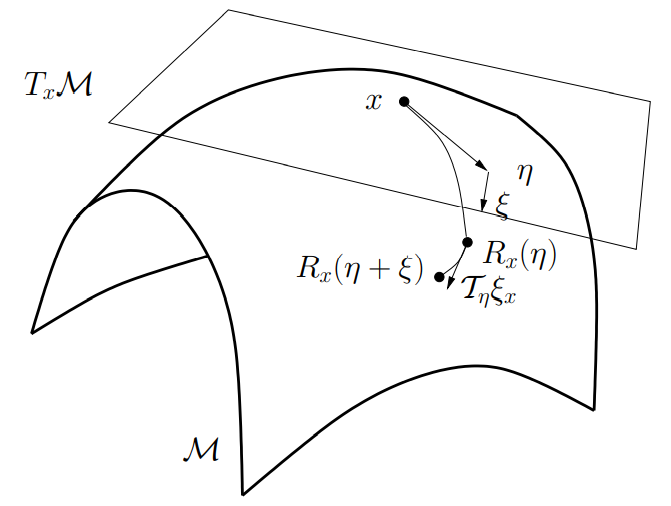
\includegraphics[width=5cm]{img/Vector_Transport_By_Differentiated.png}
        \end{tabular}
    \end{tabular}
\end{frame}
\end{comment}



\begin{frame}{Riemannian Quasi-Newton Equation}
    $\mathcal{H}_{k+1} \colon \tangent{x_{k+1}} \to \tangent{x_{k+1}}$ should... \\[0.5\baselineskip]
    ...be \textbf{self-adjoint} ($\operatorname{Hess} f(x_{k+1})$ is self-adjoint), \\[0.5\baselineskip]
    ...be \textbf{positive definite} ($\Rightarrow \eta_{k+1}$ is a descent direction) \\[0.5\baselineskip]
    ...satisfy the \textbf{Riemannian quasi-Newton} equation, 
    \begin{equation*}
            \mathcal{H}_{k+1} [T_{x_k \rightarrow x_{k+1}}({R_{x_k}}^{-1}(x_{k+1}))] = \operatorname{grad} f(x_{k+1}) - T_{x_k \rightarrow x_{k+1}}(\operatorname{grad} f(x_k)),
    \end{equation*} 
    where $R$ is the associated retraction of $T$.
\end{frame}


\begin{comment}

\begin{frame}{Riemannian Curvature Condition}
    Necessary and sufficient for the positive definite Hessian approximation is the condition
    \begin{equation*}
        g_{x_{k+1}}(s_k, y_k) = g_{x_{k+1}}(s_k, \mathcal{H}_{k+1} [s_k]) > 0.
    \end{equation*}
    In the Euclidean case, $s^{\mathrm{T}}_k y_k > 0$ is guaranteed by the second Wolfe condition 
    \begin{equation*}
        \nabla f(x_k + \alpha_k d_k)^{\mathrm{T}} d_k \geq c_2 \nabla f(x_k)^{\mathrm{T}} d_k, 
    \end{equation*}
    that is typically imposed when choosing the stepsize $\alpha_k> 0$. 
\end{frame}

\begin{frame}{Inexact Line Search}
    Generalization of the Wolfe conditions:
    \begin{equation*}
        f( R_{x_k}(\alpha_k \eta_k)) \leq f(x_k) + c_1 \alpha_k g_{x_k} (\operatorname{grad} f(x_k), \eta_k)
    \end{equation*}
    and 
    \begin{equation*}
        \frac{\mathrm{d}}{\mathrm{d}t} f(R_{x_k}(t \; \eta_k)) \vert_{t=\alpha_k} \geq c_2 \frac{\mathrm{d}}{\mathrm{d}t} f(R_{x_k}(t \; \eta_k)) \vert_{t=0},
    \end{equation*}
    or 
    \begin{equation*}
        g_{R_{x_k}(\alpha_k \eta_k)} (\operatorname{grad} f(R_{x_k}(\alpha_k \eta_k)),  T^{R}_{x_k, \alpha_k \eta_k}(\eta_k)) \geq c_2 g_{x_k} (\operatorname{grad} f(x_k), \eta_k),
    \end{equation*}
    where $0 < c_1 < c_2 < 1$ (In practice: $c_1 = 10^{-4}$ and $c_2 = 0.999$).
\end{frame}

\end{comment}

\section{(Cautious) (L-)RBFGS Method}

\begin{frame}{Riemannian BFGS Formula}
    \begin{equation*}
        \mathcal{H}^{RBFGS}_{k+1} [\cdot] = \widetilde{\mathcal{H}}^{RBFGS}_k [\cdot] + \frac{y_k y^{\flat}_k[\cdot]}{s^{\flat}_k [y_k]} - \frac{\widetilde{\mathcal{H}}^{RBFGS}_k [s_k] s^{\flat}_k (\widetilde{\mathcal{H}}^{RBFGS}_k [\cdot])}{s^{\flat}_k (\widetilde{\mathcal{H}}^{RBFGS}_k [s_k])}
    \end{equation*}
    where 
    \begin{itemize}
        \item $\widetilde{\mathcal{H}}^{RBFGS}_k = T^{S}_{x_k, \alpha_k \eta_k} \circ \mathcal{H}^{RBFGS}_k \circ {T^{S}_{x_k, \alpha_k \eta_k}}^{-1}$
        \item $s_k = T^{S}_{x_k, \alpha_k \eta_k}(\alpha_k \eta_k)$
        \item $y_k = \operatorname{grad} f(x_{k+1}) - T^{S}_{x_k, \alpha_k \eta_k}(\operatorname{grad} f(x_k))$
        \item $s^{\flat}_k \colon \tangent{x_{k+1}} \to \mathbb{R}, \;  \xi_{x_{k+1}} \mapsto s^{\flat}_k[\xi_{x_{k+1}}] = g_{x_{k+1}} (s_k, \xi_{x_{k+1}})$
    \end{itemize}
\end{frame}

\begin{frame}{Inverse Riemannian BFGS Formula}
    \begin{equation*}
        {\mathcal{H}^{RBFGS}_{k+1}}^{-1} = \mathcal{B}^{RBFGS}_{k+1} 
    \end{equation*}
    \begin{equation*}
        \begin{split}
            \mathcal{B}^{RBFGS}_{k+1} [\cdot] = & \; \widetilde{\mathcal{B}}^{RBFGS}_k [\cdot] -  \frac{s_k y^{\flat}_k[\widetilde{\mathcal{B}}^{RBFGS}_k [\cdot]]}{s^{\flat}_k [y_k]} - \frac{\widetilde{\mathcal{B}}^{RBFGS}_k [y_k]  s^{\flat}_k [\cdot]}{s^{\flat}_k [y_k]} + \\ & + \frac{y^{\flat}_k[\widetilde{\mathcal{B}}^{RBFGS}_k [y_k]] s_k s^{\flat}_k [\cdot]}{(s^{\flat}_k [y_k])^2} + \frac{s_k s^{\flat}_k [\cdot]}{s^{\flat}_k [y_k]}
        \end{split}
    \end{equation*} \\[0.3\baselineskip]
    \begin{equation*}
        \mathcal{B}^{RBFGS}_{k+1} [y_k] = s_k
    \end{equation*}
\end{frame}

\begin{frame}{Inexact Line Search}
    $\Rightarrow$ Determine a stepsize $\alpha_k > 0$ along the curve $\gamma(\alpha) = R_{x_k}(\alpha \; \eta_k)$. \\[0.3\baselineskip]
    Generalization of the \textbf{Wolfe conditions}: for $0 < c_1 < c_2 < 1$
    \begin{equation*}
        f( R_{x_k}(\alpha_k \eta_k)) \leq f(x_k) + c_1 \alpha_k g_{x_k} (\operatorname{grad} f(x_k), \eta_k)
    \end{equation*}
    and 
    \begin{equation*}
        \frac{\mathrm{d}}{\mathrm{d}t} f(R_{x_k}(t \, \eta_k)) \vert_{t=\alpha_k} \geq c_2 \frac{\mathrm{d}}{\mathrm{d}t} f(R_{x_k}(t \, \eta_k)) \vert_{t=0},
    \end{equation*}
    or 
    \begin{equation*}
        g_{R_{x_k}(\alpha_k \eta_k)} (\operatorname{grad} f(R_{x_k}(\alpha_k \eta_k)),  T^{R}_{x_k, \alpha_k \eta_k}(\eta_k)) \geq c_2 \, g_{x_k} (\operatorname{grad} f(x_k), \eta_k).
    \end{equation*}
\end{frame}

\begin{frame}{General RBFGS Method}
    \begin{algorithm}[H]
        \begin{algorithmic}[1]
            \State $x_0 \in \mathcal{M}$, $\mathcal{B}^{RBFGS}_0 \colon \tangent{x_0} \to \tangent{x_0}$.
            \While{not converged}
            \State Set $\eta_k = - \mathcal{B}^{RBFGS}_k [\operatorname{grad} f(x_k)]$.
            \State Determine $\alpha_k > 0$ that satisfies Wolfe conditions. 
            \State Set $x_{k+1} = R_{x_k}(\alpha_k \eta_k)$.
            \State Update $\mathcal{B}^{RBFGS}_k \mapsto \mathcal{B}^{RBFGS}_{k+1} \colon \tangent{x_{k+1}} \to \tangent{x_{k+1}}$. 
            \State $k = k+1$.
        \EndWhile
        \end{algorithmic}
    \end{algorithm}
\end{frame}

\begin{frame}{Positive Definite Update}
    \begin{itemize}
        \item If $g_{x_{k+1}}(s_k, y_k) > 0$, then $\mathcal{B}^{RBFGS}_{k+1}$ is self-adjoint and positive definite if and only if $\mathcal{B}^{RBFGS}_k$ is self-adjoint and positive definite: \begin{equation*}\mathcal{B}^{RBFGS}_0 = \kappa \, id_{\tangent{x_0}}, \quad \kappa > 0.\end{equation*}
        \item But $g_{x_{k+1}}(s_k, y_k) > 0$ is \textbf{not guaranteed by the second Wolfe condition}, since $T^R \neq T^S$.
    \end{itemize}
    \vspace{9.5pt}
    $\Rightarrow$ \textbf{Restrictions on retraction and vector transport must be made}.
\end{frame}



\begin{comment}

\begin{frame}{Geodesics}
    \begin{tabular}{cl}  
        \begin{tabular}{c}
            \parbox{0.4\linewidth}
            {
                Curve $\gamma \colon \; I \to \mathcal{M}$,  with zero acceleration:
                \begin{equation*}
                    \frac{\mathrm{D}^2}{\mathrm{d}t^2} \gamma(t) = \nabla_{\dot{\gamma}(t)} \dot{\gamma}(t) = 0, \; \forall t \in I.
                \end{equation*}
                $\Rightarrow \lVert \dot{\gamma}(t) \rVert_{\gamma(t)} = c$ 
            }
        \end{tabular}  
        &
        \begin{tabular}{l}
            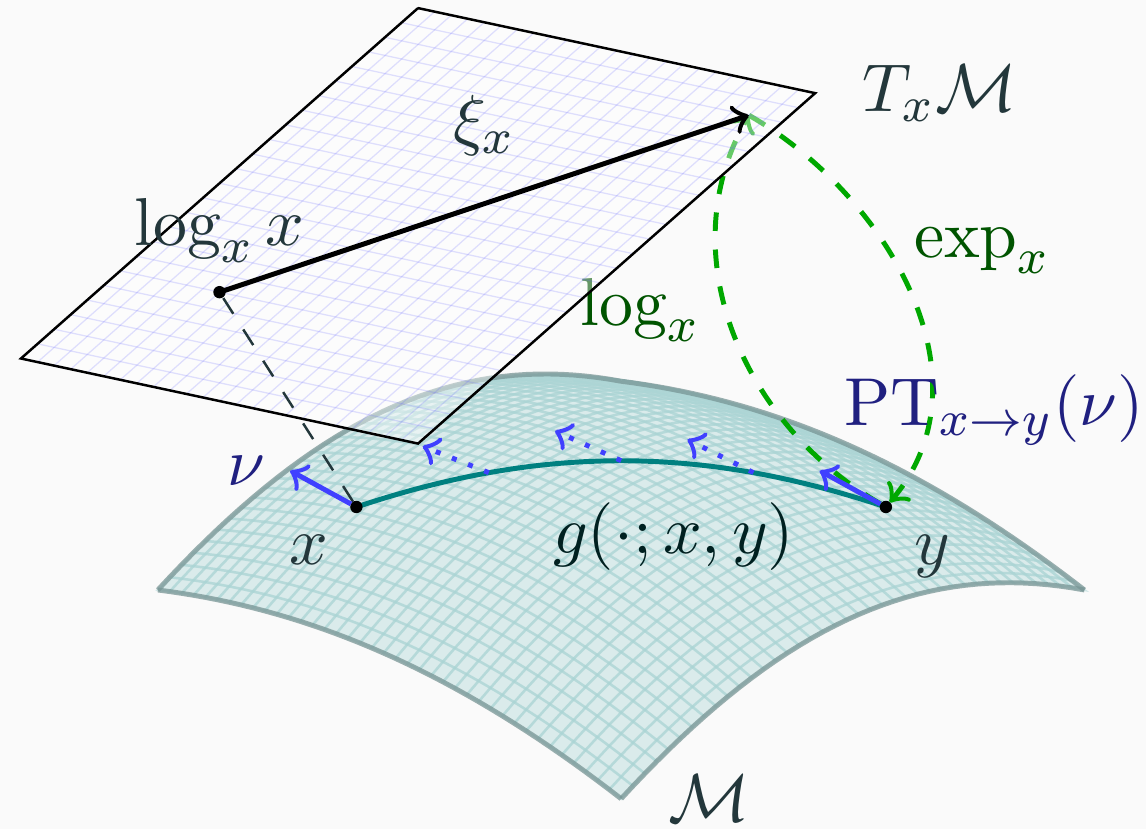
\includegraphics[width=6cm]{img/Manifold-Illustration.png}
        \end{tabular}
    \end{tabular}
\end{frame}

\begin{frame}{Exponential Map and Parallel Transport}
    \begin{tabular}{cl}  
        \begin{tabular}{c}
            \parbox{0.4\linewidth}
            {
                \begin{equation*}
                    \begin{split}
                        \exponential{x} \colon \; \tangent{x} & \to \mathcal{M} \\
                        \xi_x & \mapsto \exponential{x}(\xi_x) = \gamma_{\xi_x}(1)
                    \end{split}
                \end{equation*}
                \begin{equation*}
                    \begin{split}
                        \mathrm{PT}_{x, \xi_x} \colon \; \tangent{x} & \to \tangent{\exponential{x}(\xi_x)} \\
                        \eta_x & \mapsto \mathrm{PT}_{x, \xi_x}(\eta_x)
                    \end{split}
                \end{equation*}
            }
        \end{tabular}  
        &
        \begin{tabular}{l}
            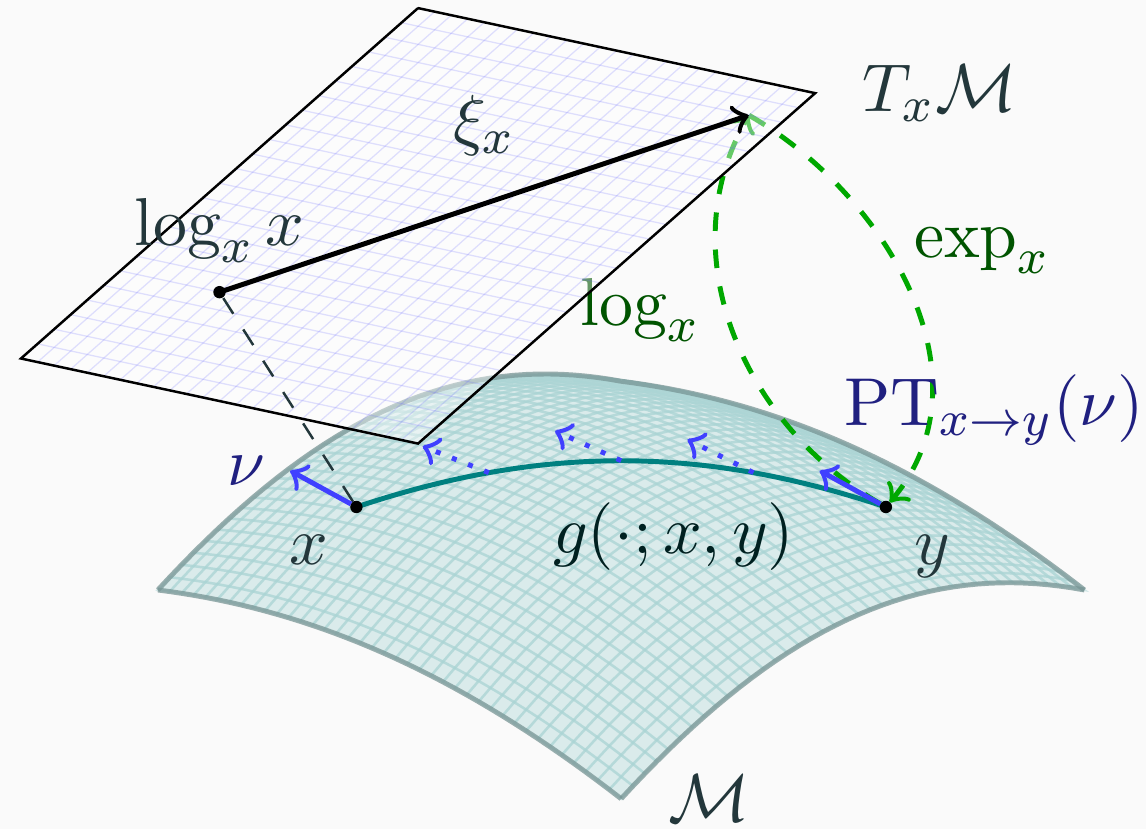
\includegraphics[width=6cm]{img/Manifold-Illustration.png}
        \end{tabular}
    \end{tabular}

\end{frame}  
\end{comment}

\begin{frame}{RBFGS with $\expOp$ and $\mathrm{PT}$}
    \vspace{-1\baselineskip}\hfill{\tiny{[Qi, 2011]}}
    \begin{equation*}
        x_{k+1} = \exponential{x_k}(\alpha_k \eta_k)
    \end{equation*}
    \begin{itemize}
        \item $\widetilde{\mathcal{B}}^{RBFGS}_k = \mathrm{PT}_{x_k, \alpha_k \eta_k} \circ \mathcal{B}^{RBFGS}_k \circ {\mathrm{PT}_{x_k, \alpha_k \eta_k}}^{-1}$
        \item $s_k = \mathrm{PT}_{x_k, \alpha_k \eta_k}(\alpha_k \eta_k)$
        \item $y_k = \operatorname{grad} f(x_{k+1}) - \mathrm{PT}_{x_k, \alpha_k \eta_k}(\operatorname{grad} f(x_k))$
    \end{itemize}
\end{frame}


\begin{comment}
\begin{frame}{Initialization}
    \begin{itemize}
        \item An initial iterate $x_0 \in \mathcal{M}$.
        \item An initial positive definite and self-adjoint operator $\mathcal{B}^{RBFGS}_0 \colon \; \tangent{x_0} \to \tangent{x_0}$.
        \item Line search parameters $0 < c_1 < \frac{1}{2} < c_2 < 1$.
    \end{itemize}
    In practice:
    \begin{itemize}
        \item $\mathcal{B}^{RBFGS}_0 = id_{\tangent{x_0}}$
        \item $c_1 = 10^{-4}$ and $c_2 = 0.999$
    \end{itemize}
\end{frame}

\begin{frame}
    \begin{algorithm}[H]
        \begin{algorithmic}[1]
            \While{not converged}
            \State $\eta_k = - \mathcal{B}^{RBFGS}_k [\operatorname{grad} f(x_k)]$.
            \State Determine a stepsize $\alpha_k > 0$ that satisfies the Wolfe conditions. 
            \State $x_{k+1} = \exponential{x_k} (\alpha_k \eta_k)$.
            \State Define $\widetilde{\mathcal{B}}^{RBFGS}_k$, $s_k$ and $y_k$.
            \State Compute $\mathcal{B}^{RBFGS}_{k+1} \colon \; \tangent{x_{k+1}} \to \tangent{x_{k+1}}$. 
            \State $k = k+1$.
        \EndWhile
        \State \textbf{Return} $x_k$.
        \end{algorithmic}
    \end{algorithm}
\end{frame}

\begin{frame}{Properties}
    \begin{itemize}
        \item The statements about convergence known in the Euclidean case can be generalized $\Rightarrow$ global convergence for twice continuously differentiable convex objective functions and superlinear convergence under additional assumptions can be shown.
        \item For some manifolds, either the exponential map, $\expOp$, or the parallel transport, $\mathrm{PT}$, are not available or are computationally too costly.
    \end{itemize}
\end{frame}
\end{comment}


\begin{frame}{RBFGS with Locking Condition}
    \vspace{-1\baselineskip}\hfill{\tiny{[Huang, Gallivan, Absil, 2015]}} \\
    $T^S$ with associated $R$ satisfies $\forall \xi_x \in \tangent{x}$ and $\forall x \in \mathcal{M}$
    \begin{equation*}
        T^{S}_{x, \xi_x}(\xi_x) = \beta \; T^{R}_{x, \xi_x}(\xi_x), \quad \beta = \frac{\lVert \xi_x \rVert_x}{\lVert T^{R}_{x, \xi_x}(\xi_x) \rVert_{R_{x}(\xi_x)}}.
    \end{equation*} \\[0.3\baselineskip]
    \begin{equation*}
        \Rightarrow x_{k+1} = R_{x_k}(\alpha_k \eta_k), \widetilde{\mathcal{B}}^{RBFGS}_k, s_k \text{ as usual, but}
    \end{equation*}
    \begin{equation*}
        y_k = {\beta_k}^{-1} \, \operatorname{grad} f(x_{k+1}) - T^{S}_{x_k, \alpha_k \eta_k}(\operatorname{grad} f(x_k)),
    \end{equation*}
    \begin{equation*}
        \text{where} \quad \beta_k = \frac{\lVert \alpha_k \eta_k \rVert_{x_k}}{\lVert T^{R}_{x_k, \alpha_k \eta_k}(\alpha_k \eta_k) \rVert_{x_{k+1}}}.
    \end{equation*}
\end{frame}


\begin{comment}
\begin{frame}{(Additional) Initialization}
    \begin{itemize}
        \item $x_0 \in \mathcal{M}$, $\mathcal{B}^{RBFGS}_k$, $0 < c_1 < \frac{1}{2} < c_2 < 1$ as before.
        \item An isometric vector transport $T^S$ with $R$ as associated retraction, which satisfies the locking condition. 
    \end{itemize}
\end{frame}

\begin{frame}
    \begin{algorithm}[H]
        \begin{algorithmic}[1]
            \While{not converged}
            \State $\eta_k = - \mathcal{B}^{RBFGS}_k [\operatorname{grad} f(x_k)]$.
            \State Determine a stepsize $\alpha_k > 0$ that satisfies the Wolfe conditions. 
            \State $\color{red} x_{k+1} = R_{x_k}(\alpha_k \eta_k)$.
            \State Define $\color{red} \widetilde{\mathcal{B}}^{RBFGS}_k$, $\color{red} s_k$ and $\color{red} y_k$.
            \State Compute $\mathcal{B}^{RBFGS}_{k+1} \colon \; \tangent{x_{k+1}} \to \tangent{x_{k+1}}$. 
            \State $k = k+1$.
        \EndWhile
        \State \textbf{Return} $x_k$.
        \end{algorithmic}
    \end{algorithm}
\end{frame}


\begin{frame}{Properties}
    \begin{itemize}
        \item If $f$ is twice continuously differentiable and strongly retraction-convex ($t \mapsto R_x(t \eta_x)$ is strongly convex) $\Rightarrow$ global convergence.
        \item Superlinear convergence can be shown. 
    \end{itemize}
\end{frame}
\end{comment}


\begin{frame}{Weak line search conditions}
    \vspace{-1\baselineskip}\hfill{\tiny{[Huang, Absil, Gallivan, 2018]}} \\
    For $0 < \chi_1, \chi_2 < 1$:
    \begin{equation}
        f(R_{x_k}(\alpha_k \eta_k)) - f(x_k) \leq - \chi_1 \, \frac{{g_{x_k} (\operatorname{grad} f(x_k), \eta_k)}^2}{\lVert \eta_k \rVert^2_{x_k}}
    \end{equation} 
    \textbf{or}
    \begin{equation}
        f(R_{x_k}(\alpha_k \eta_k)) - f(x_k) \leq \chi_2 \, g_{x_k} (\operatorname{grad} f(x_k), \eta_k).
    \end{equation} \\[1.\baselineskip]
    $\Rightarrow$ $T^R$ is not needed!
\end{frame}


\begin{frame}{Cautious RBFGS}
    \vspace{-1\baselineskip}\hfill{\tiny{[Huang, Absil, Gallivan, 2018]}}\\
    \begin{equation*}
        x_{k+1} = R_{x_k}(\alpha_k \eta_k),
    \end{equation*}
    where $\alpha_k$ satisfies (1) \textbf{or} (2). \\[.5\baselineskip]
    \begin{equation*}
        \mathcal{B}^{CRBFGS}_{k+1} = \begin{cases} \mathcal{B}^{RBFGS}_{k+1}, & \; \frac{g_{x_{k+1}}(y_k,s_k)}{\lVert s_k \rVert^{2}_{x_{k+1}}} \geq \theta(\lVert \operatorname{grad} f(x_k) \rVert_{x_k}), \\ \widetilde{\mathcal{B}}^{CRBFGS}_k, & \; \text{otherwise}, \end{cases}
    \end{equation*}
    where $\theta$ is a monotone increasing function satisfying $\theta(0) = 0$ and $\theta$ is strictly increasing at $0$. \\[.5\baselineskip]
    $\Rightarrow$ All operators $\{\mathcal{B}^{CRBFGS}_k\}_k$ are \textbf{positive definite}!
\end{frame}



\begin{comment}
\begin{frame}{Initialization}
    \begin{itemize}
        \item $x_0 \in \mathcal{M}$, $\mathcal{B}^{CRBFGS}_0$, as before.
        \item An isometric vector transport $T^S$ with $R$ as associated retraction. 
        \item Line search parameters $0 < \chi_1, \chi_2 < 1$.
        \item A monotone increasing function satisfying $\theta(0) = 0$ and $\theta$ is strictly increasing at $0$.
    \end{itemize}
\end{frame}

\begin{frame}
    \begin{algorithm}[H]
        \begin{algorithmic}[1]
            \While{not converged}
            \State $\eta_k = - \mathcal{B}^{CRBFGS}_k [\operatorname{grad} f(x_k)]$.
            \State Determine a stepsize $\color{red} \alpha_k > 0$ that satisfies the weak line search conditions. 
            \State $x_{k+1} = R_{x_k}(\alpha_k \eta_k)$.
            \State Define $\widetilde{\mathcal{B}}^{RBFGS}_k$, $s_k$ and $y_k$.
            \State Compute $\color{red} \mathcal{B}^{CRBFGS}_{k+1} \colon \; \tangent{x_{k+1}} \to \tangent{x_{k+1}}$. 
            \State $k = k+1$.
        \EndWhile
        \State \textbf{Return} $x_k$.
        \end{algorithmic}
    \end{algorithm}
\end{frame}


\begin{frame}{Properties}
    \begin{itemize}
        \item The iterates $\{ x_k \}$ satisfy $\liminf_{k \to \infty} \lVert \operatorname{grad} f(x_k) \rVert_{x_k} = 0$.
        \item Under some reasonable assumptions, the cautious RBFGS update reduces to the ordinary RBFGS update around a non-degenerate minimizer, i.e. $\mathcal{B}^{CRBFGS}_{k+1} = \mathcal{B}^{RBFGS}_{k+1}$ and superlinear convergence follows.
    \end{itemize}
\end{frame}

\end{comment}

\begin{frame}{Limited-Memory RBFGS}
    \begin{center}
        $\mathcal{B}^{RBFGS}_{k+1}  = \mathcal{V}^{\flat}_k \circ \widetilde{\mathcal{B}}^{RBFGS}_k \circ \mathcal{V}_k [\cdot] + \rho_k s_k s_k^{\flat} [\cdot]$\\[1.\baselineskip]

        $\rho_k = \frac{1}{g_{x_{k+1}}(s_k, y_k)} , \quad \mathcal{V}_k [\cdot] = \mathrm{id}_{\tangent{x_{k+1}}}[\cdot] - \rho_k y_k s^{\flat}_k [\cdot]$ \\[1.\baselineskip]

        $\mathcal{B}^{LRBFGS}_k [\cdot] = \mathcal{B}^{(m)}_k [\cdot] =  \mathcal{V}^{\flat}_{k-1} \circ \widetilde{\mathcal{B}}^{(m-1)}_k \circ \mathcal{V}_{k-1} [\cdot] + \rho_{k-1} s_{k-1} s_{k-1}^{\flat} [\cdot]$\\[1.\baselineskip]

        $\mathcal{B}^{(0)}_k = \frac{g_{x_k}(s_{k-1}, y_{k-1})}{g_{x_k}(y_{k-1}, y_{k-1})} \; \mathrm{id}_{\tangent{x_k}}, \quad \{ \widetilde{s}_i, \widetilde{y}_i\}_{i=k-m}^{k-1} \subset \tangent{x_k}$
    \end{center}
\end{frame}


\begin{comment}
\begin{frame}{LRBFGS Two-Loop Recursion for $\mathcal{B}^{LRBFGS}_k[\operatorname{grad} f(x_k)]$}
    \begin{algorithm}[H]
        \begin{algorithmic}[1]
            \State $q = \operatorname{grad} f(x_k)$
            
            \For{$i = k-1, k-2, \cdots, k-m$}
                \State $\rho_i = \frac{1}{g_{x_k}(\widetilde{s}_i, \widetilde{y}_i)}$
                \State $\xi_i = \rho_i g_{x_k}(\widetilde{s}_i, q)$ 
                \State $q = q - \xi_i \widetilde{y}_i$
            \EndFor
    
            \State $r = \mathcal{B}^{(0)}_k[q]$
            
            \For{$i = k-m, k-m+1, \cdots, k-1$}
                \State $\omega = \rho_i g_{x_k}(\widetilde{y}_i, r)$ 
                \State $r= r  + (\xi_i - \omega) \widetilde{s}_i$
            \EndFor
            
            \State \textbf{Stop with result} $\mathcal{B}^{LRBFGS}_k[\operatorname{grad} f(x_k)]$.
        \end{algorithmic}
    \end{algorithm}
\end{frame}
\end{comment}

\begin{frame}
    \begin{algorithm}[H]
        \begin{algorithmic}[1]
            \While{not converged}
            \State $\eta_k = - \mathcal{B}^{LRBFGS}_k [\operatorname{grad} f(x_k)]$ by Two-Loop Recursion.
            \State Determine $\alpha_k > 0$ that satisfies Wolfe conditions. 
            \State Set $x_{k+1} = R_{x_k}(\alpha_k \eta_k)$.
            \If{$k > m$}
                \State Discard $\{ \widetilde{s}_{k-m}, \widetilde{y}_{k-m}\}$, $T^{S}_{x_k, \alpha_k \eta_k} (\{ \widetilde{s}_i, \widetilde{y}_i\}_{i=k-m+1}^{k-1})$.
			\Else 
				\State $T^{S}_{x_k, \alpha_k \eta_k} (\{ \widetilde{s}_i, \widetilde{y}_i\}_{i=k-m+1}^{k-1})$.
            \EndIf 
            \State Add $s_k = \widetilde{s}_k$ and $y_k = \widetilde{y}_k$ into storage.
            \State $k = k+1$.
        \EndWhile
        \State \textbf{Return} $x_k$.
        \end{algorithmic}
    \end{algorithm}
\end{frame}

\section{Numerics}

\begin{comment}
\begin{frame}{Bases and Coordinate Expressions}
    \begin{center}
        $\tangent{x}$ is a $n$-dimensional vector space $\Rightarrow$ existence of an orthonormal basis $(e_1, \cdots, e_n)$ in $\tangent{x}$: \\[1.\baselineskip]

        $\xi_x = \xi^{1}_x e_1 + \cdots + \xi^{n}_x e_n \in \tangent{x}$ with $\hat{\xi_x} = (\xi^{1}_x, \cdots, \xi^{n}_x) \in \mathbb{R}^n$ \\[1.\baselineskip]

        $G_x = (g_x(e_i, e_j))^{n}_{i,j=1} = I_{n \times n} \in \mathrm{R}^{n \times n}$ \\[1.\baselineskip]

        $\Rightarrow g_x(\xi_x, \eta_x) = \hat{\xi_x}^{\mathrm{T}} G_x \hat{\eta_x} = \hat{\xi_x}^{\mathrm{T}} \hat{\eta_x}$ \\[1.\baselineskip]

        $\mathcal{B} [\xi_x] = (\hat{\mathcal{B}}\hat{\xi_x})_1 e_1 + \cdots + (\hat{\mathcal{B}}\hat{\xi_x})_n e_n \in \tangent{x}$
    \end{center}
\end{frame}


\begin{frame}{Realizing the RBFGS Formula}
    Create ONB $(e_1, \cdots, e_n) \subset \tangent{x_0}$ and $\mathcal{B}^{RBFGS}_0 \simeq B^{RBFGS}_0 = \kappa \, I_{n \times n}$. \\[1.\baselineskip]
    \begin{itemize}
        \item $\operatorname{grad} f(x_k) \mapsto \widehat{\operatorname{grad} f(x_k)} \in \mathbb{R}^n$.
        \item $B^{RBFGS}_k \widehat{\operatorname{grad} f(x_k)} = \hat{\eta_k} \mapsto \eta_k \in \tangent{x_k}$.
        \item $x_{k+1}$, $s_k$, $y_k$ as usual.
        \item $s_k, y_k \mapsto \hat{s_k}, \hat{y_k}$. We note $\hat{s_k}^{\mathrm{T}} \hat{y_k} > 0$.
        \item $B^{RBFGS}_k \rightarrow B^{RBFGS}_{k+1}$ (Euclidean Update).
    \end{itemize}
\end{frame}
\end{comment}

\begin{frame}{Manopt.jl}
    \begin{center}
        
\includegraphics[width=8cm]{img/quasi_Newton_call.png} \\[.5\baselineskip]
    \end{center}
    Optional input arguments:
    \begin{itemize}
        \item Memory size ($20$, if $<0 \Rightarrow$ RBFGS)
        \item Retraction ($\expOp$)
        \item Vector transport ($\mathrm{PT}$)
        \item Cautious update (not used) \\[.5\baselineskip]
    \end{itemize}
    $\Rightarrow$ \textbf{LRBFGS with a memory size of $20$, using $\expOp$ and $\mathrm{PT}$}. 
\end{frame}

\begin{frame}{Rayleigh Quotient Minimization}
    $A \in \mathbb{R}^{n \times n}$ symmetric, the unit-norm eigenvector, $v \in \mathbb{R}^n$, corresponding to the smallest eigenvalue, defines the two global minima, $\pm v$, of the Rayleigh quotient  
    \begin{equation*}
        \begin{split}
            f \colon \; \mathbb{S}^{n-1} & \to \mathbb{R} \\
            x & \mapsto x^{\mathrm{T}} A x 
        \end{split}
    \end{equation*}   
    with its Riemannian gradient \\[.3\baselineskip]
    \begin{equation*}
        \operatorname{grad} f(x) = 2(Ax - x x^{\mathrm{T}} A x).
    \end{equation*}
\end{frame}

\begin{frame}{Experiment}
    \begin{center}
        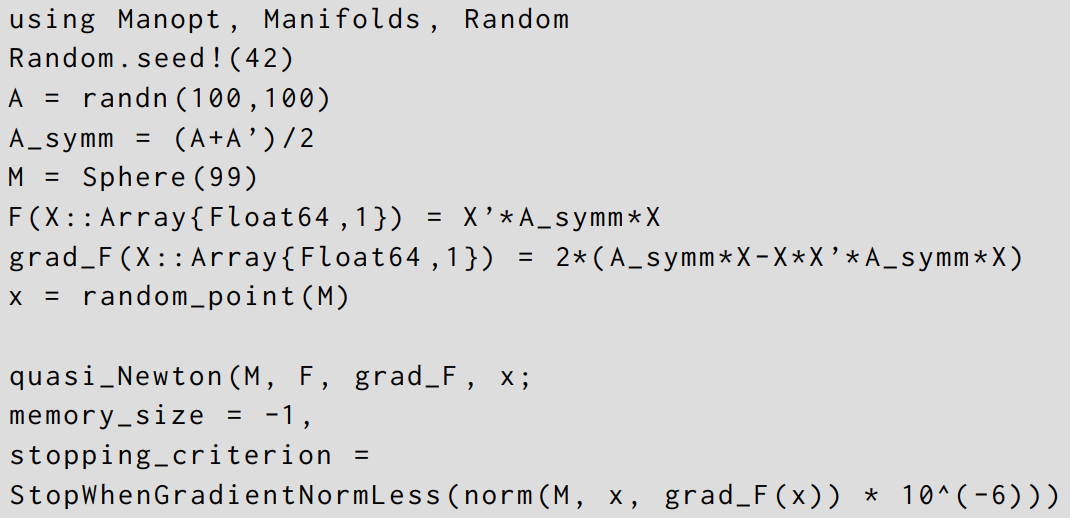
\includegraphics[width=11cm]{img/Rayleigh.png}
    \end{center}
\end{frame}

\begin{frame}{Results}
    Comparison of RBFGS from Manopt.jl with RBFGS from [Qi, 2011] in an average of 10 random runs:
    \begin{table}[H]
        \resizebox{\textwidth}{!}{
            \begin{tabular}{l l l l l }
                \toprule
                Manifold & \multicolumn{2}{c}{$\mathbb{S}^{99}$}& \multicolumn{2}{c}{$\mathbb{S}^{299}$} \\ 
                \midrule
                Software & Julia & Matlab & Julia & Matlab  \\ 
                \midrule
                Time in seconds & $0.15$ & $0.54$ & $0.96$ & $11.0$ \\ 
                \midrule
                Iterations & $72$ & $72$ & $70$ & $97$ \\
                \bottomrule
            \end{tabular}
        }
    \end{table}
\end{frame}

\section{Conclusion}

\begin{frame}{Conclusion}
    \begin{itemize}
        \item The BFGS method and variants thereof are generalized to Riemannian manifolds.
        \item Right choice of vector transport and retraction is important!
        \item RBFGS methods are implemented in Manopt.jl.
        \item LRBFGS needs a lot of allocations $\Rightarrow$ very slow!
    \end{itemize}
    \begin{center}
        Thank you for your attention! Questions? 
    \end{center}
\end{frame}


\begin{comment}

\begin{frame}
    \begin{center}
        Thank you for your attention and I wish you a 
        \begin{equation*}
            \begin{split}
                y & = \frac{\log_{e}(\frac{x}{m} - as)}{r^2} \\
                r^2 y & = \log_{e}(\frac{x}{m} - as) \\
                e^{r^2 y} & = \frac{x}{m} - as \\
                m \, e^{r r y} & = x - mas.
            \end{split}
        \end{equation*}
        \begin{center}
            Questions?
        \end{center}
    \end{center}
\end{frame}
    
\end{comment}

\end{document}
